% !TeX root = ../main.tex

\xchapter{绪论}{Introduction}

\xsection{研究背景与意义}{Background and Motivation}

近年来，以深度学习为代表的人工智能技术快速发展，尤其是以Transformer为核心架构的大语言模型推动了云端与端侧推理需求的爆发式增长\cite{vaswani2017attention,zhao2023llm_survey}。在算力需求持续攀升、制程红利逐步放缓的背景下，神经网络处理器（Neural Network Processor Unit, NPU）等领域专用架构（Domain Specific Architecture, DSA）芯片成为提升性能与能效的重要路径\cite{hennessy2019golden}。多核 NPU 在扩展峰值算力的同时，其系统级行为受存储带宽、片上互连与编译调度策略复杂度的联合约束，在设计阶段就需对架构参数与映射策略进行联合评估与探索。

\xsubsection{人工智能发展与神经网络芯片算力演进}{AI Progress and NPU Performance Trends}

人工智能的发展呈现出模型规模与任务复杂度持续上升的态势。从早期卷积网络到 Transformer 与大语言模型，参数量与训练算力需求呈指数级增长。为应对这一趋势，产业界持续推出新一代 NPU 与其他 DSA 芯片，其峰值算力与能效在代际迭代中不断提升，与上层模型创新形成相互牵引。图\ref{fig:c1_npu_performance_timeline} 给出典型神经网络模型演进与 NPU 峰值性能随时间变化的示意时间线，表明硬件代际与模型形态在较长时间尺度上同步推进。图\ref{fig:c1_dl_training_compute} 给出深度神经网络所需训练算力随发布年份的指数级增长趋势，直观反映大模型发展对算力需求的持续攀升\cite{sastry2024computing}。模型—硬件与训练算力两条线索共同说明：AI 工作负载的演进不断抬高对专用算力的需求，而 NPU 芯片则通过工艺、架构与多核横向扩展持续提高芯片算力。

\begin{figure}[htbp]
  \centering
  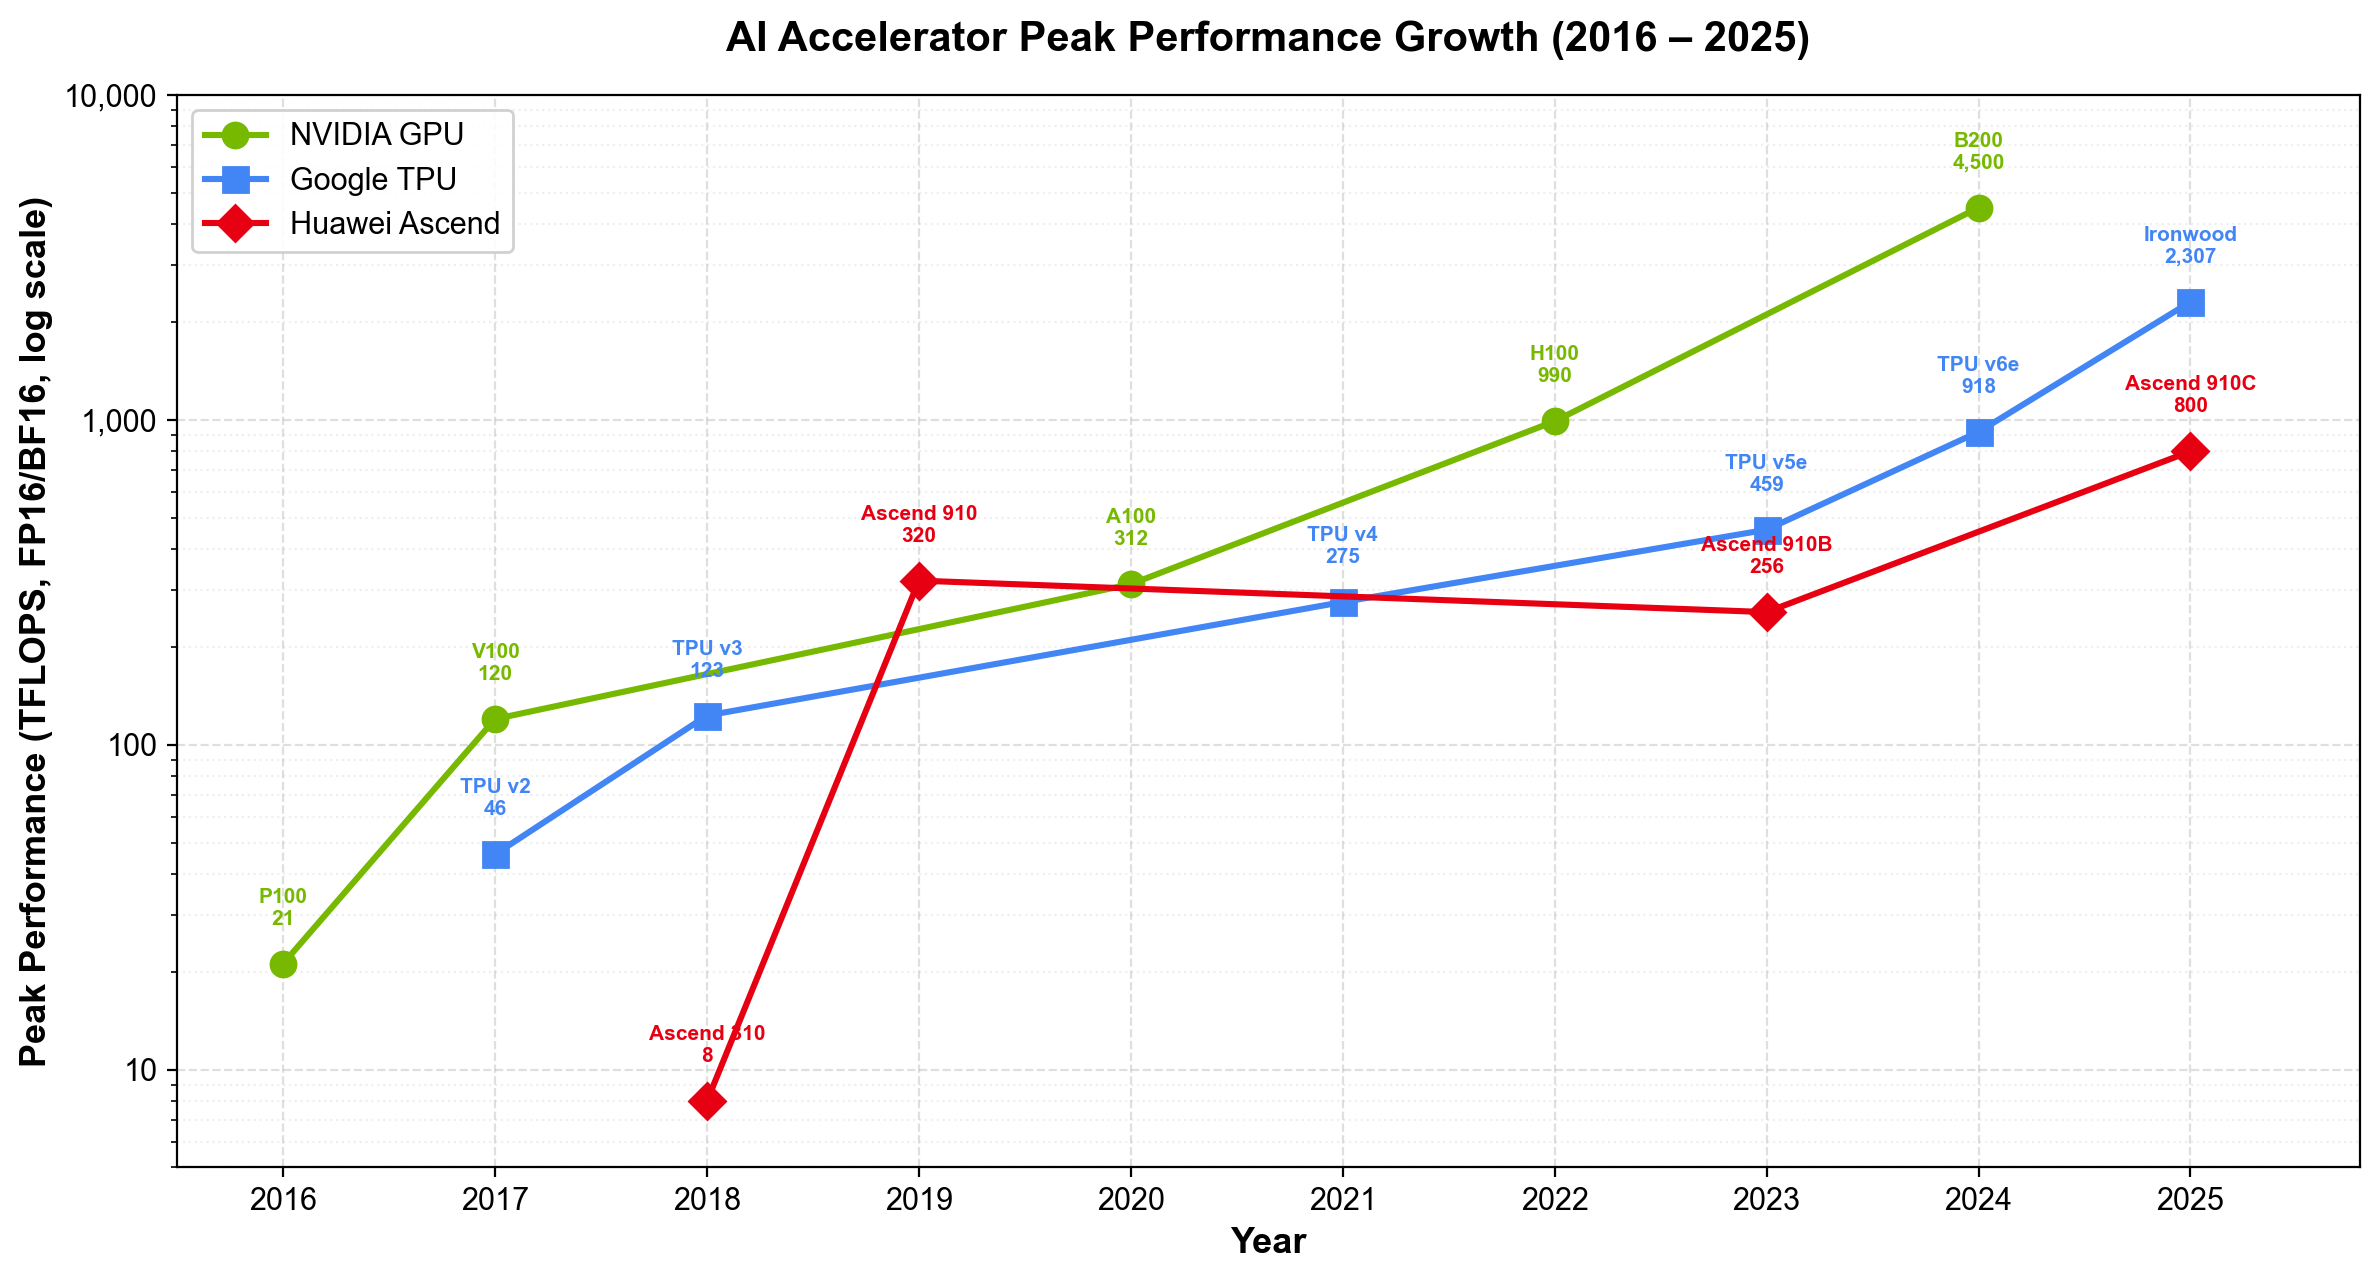
\includegraphics[width=0.78\textwidth,height=0.34\textheight,keepaspectratio]{Figures/npu_performance_timeline.png}
  \caption{典型神经网络芯片峰值性能随时间的变化（示意）。}
  \label{fig:c1_npu_performance_timeline}
\end{figure}

\begin{figure}[htbp]
  \centering
  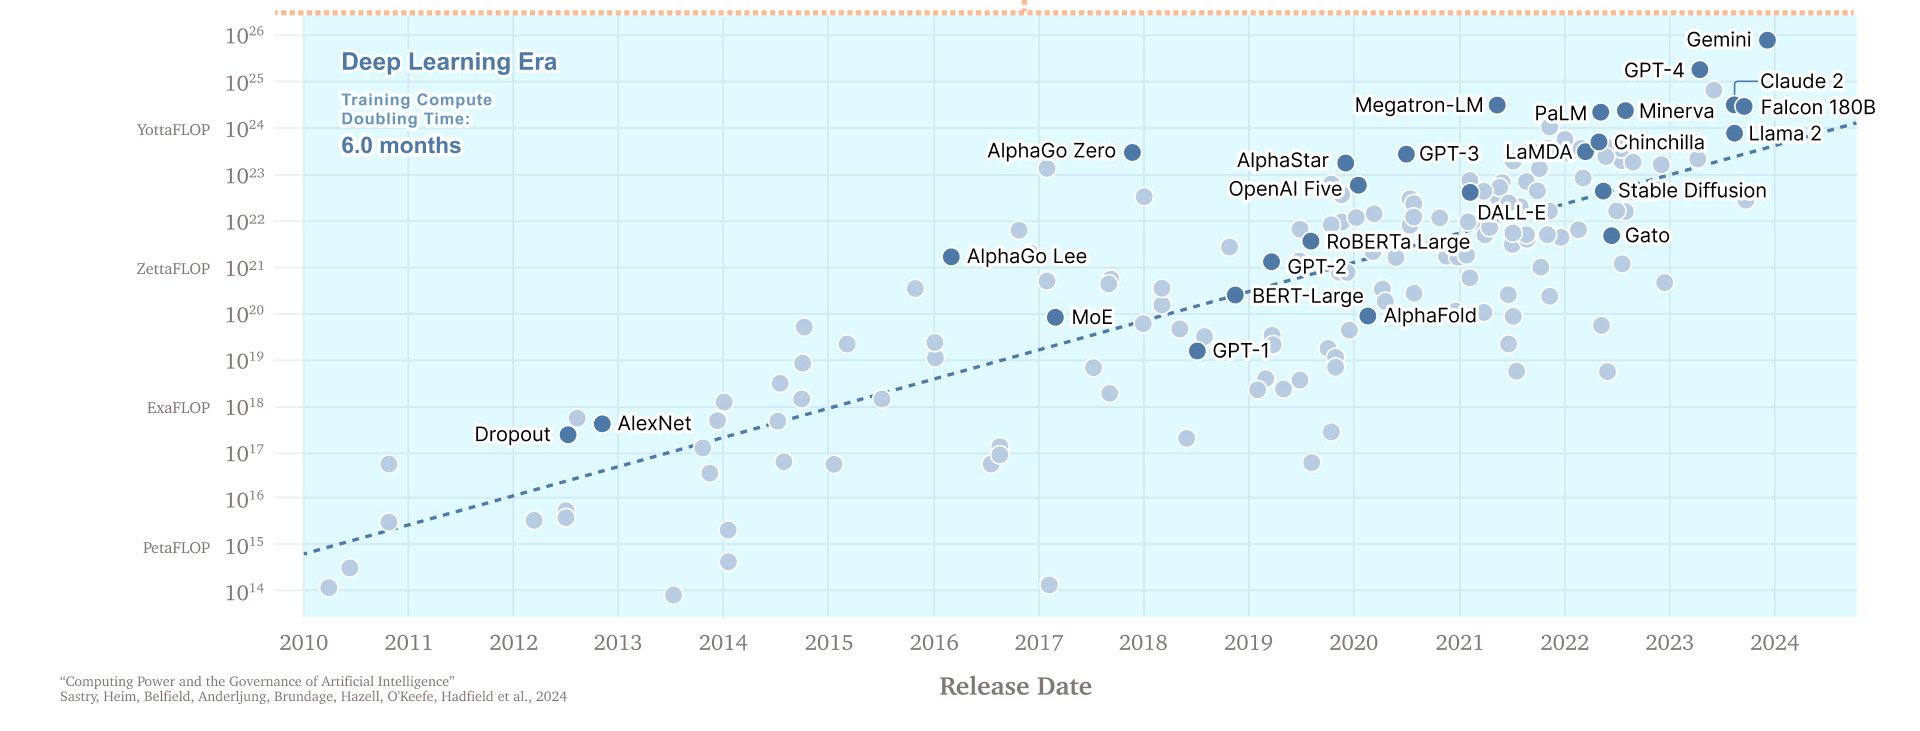
\includegraphics[width=\textwidth]{Figures/dl_training_compute.jpg}
  \caption{神经网络模型训练所需算力随发布年份的增长趋势（训练算力约每 6 个月翻倍）。图片来源：Sastry et al.\cite{sastry2024computing}（arXiv:2402.08797）。}
  \label{fig:c1_dl_training_compute}
\end{figure}

NPU 是面向神经网络推理与训练而设计的专用加速器，通常具备高并行度的矩阵/向量运算单元、层次化片上存储以及面向数据流的访存与调度机制，与通用 CPU/GPU 在编程模型与能效比上形成差异化补充。国内外已有多款代表性 NPU 芯片落地。例如 Google 的 TPU 系列在云端推理与训练场景中采用脉动阵列作为计算单元的核心架构。华为昇腾、寒武纪思元等国产 NPU 在云端与边缘端部署中兼顾多核扩展与软件栈生态。NVIDIA 的推理加速方案（如 NVDLA 等）则与已有 GPU 生态形成协同。Cerebras 则是超大算力多核NPU的代表产品（如图\ref{fig:c1_cerebras} ），将整片晶圆集成为单一大规模计算平面，将多核扩展推向物理极限。这些芯片在单核算力、多核互联与存储层次上形态各异，但共同面临算力增长时的系统级瓶颈问题。随着单芯片算力规模受限，多核阵列成为扩展 NPU 算力与兼顾能效的主流方向，但也引入了片上网络拥塞、主存带宽瓶颈与跨核调度复杂度高等系统级挑战\cite{reuther2024memorywall,cai2024gemini}。

在先进工艺下，芯片的流片成本高昂且迭代周期长。为了在设计早期进行架构探索与软硬件协同优化，构建端到端、高保真且可扩展的多核NPU模拟平台具有重要意义。一方面，周期级模拟能够在统一时间轴下刻画计算、通信与存储的竞争行为，从而定位端到端性能瓶颈。另一方面，模拟平台为映射策略、互连配置与存储参数的设计空间探索（Design Space Exploration，DSE）提供低成本试错环境\cite{jin2024onnxim,luo2023ramulator2}。从单核到多核阵列、单芯片再到晶圆级形态，算力扩展不断伴随着系统级瓶颈。

\begin{figure}[htbp]
  \centering
  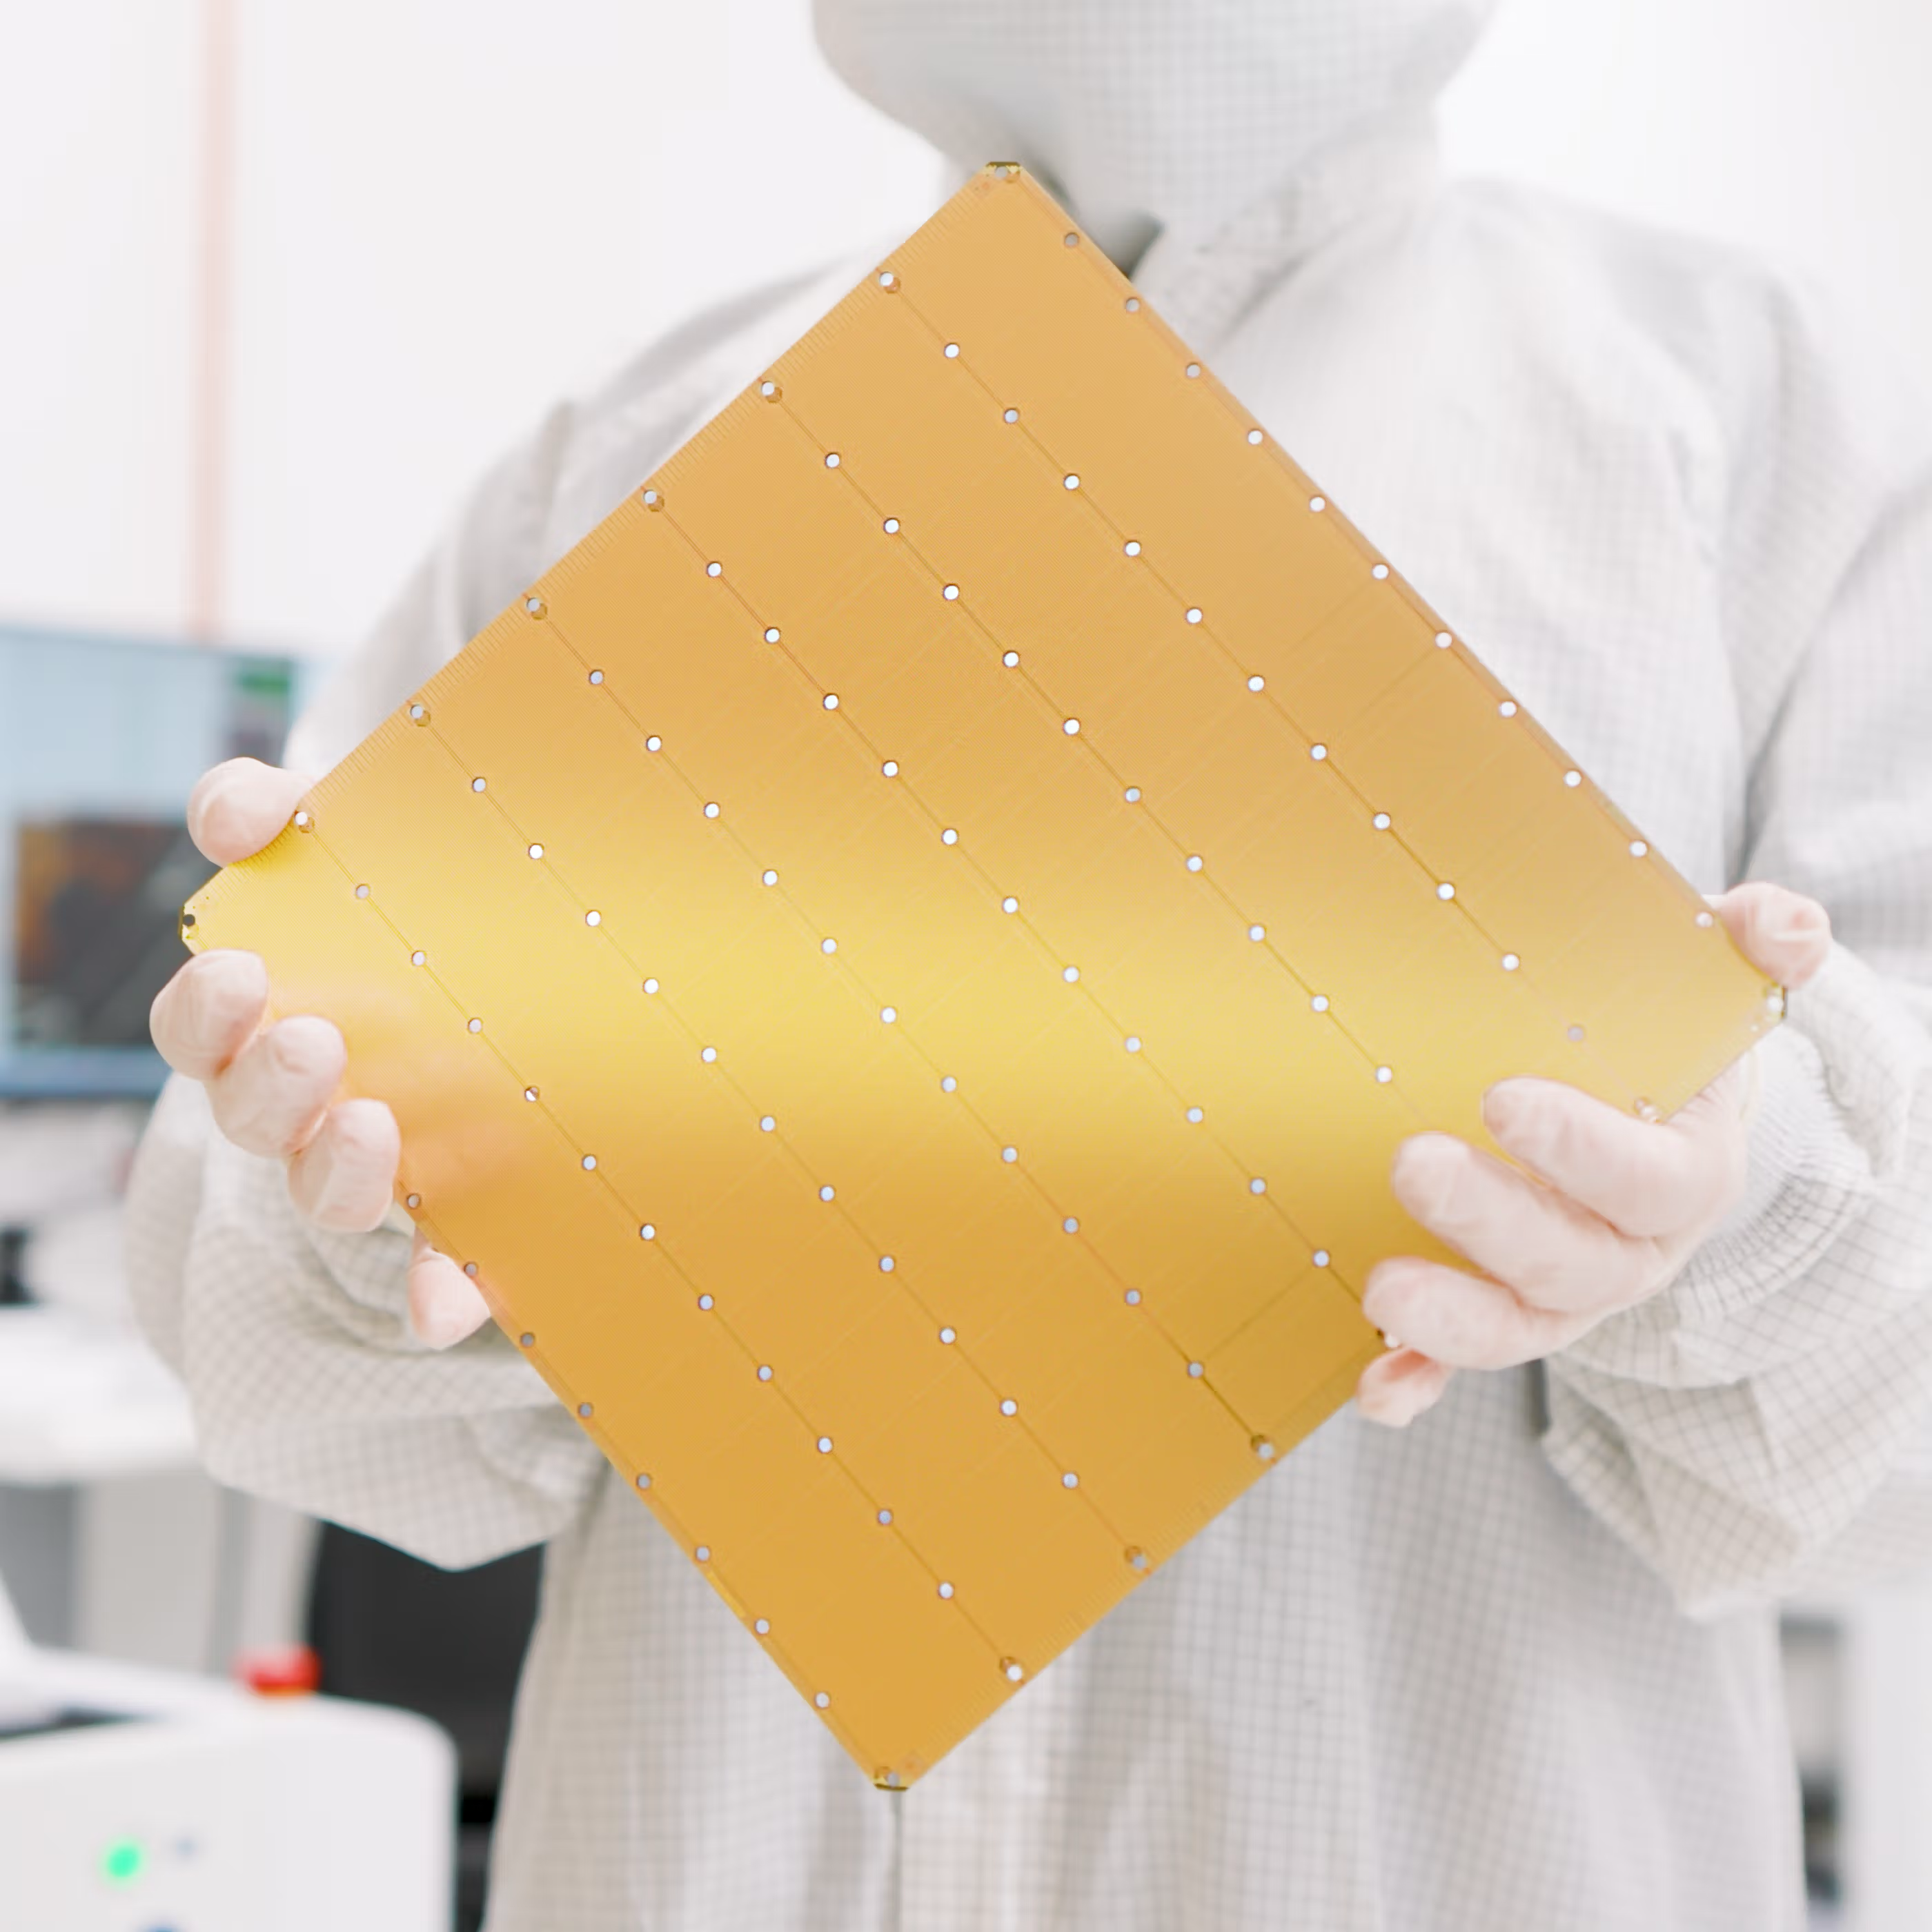
\includegraphics[width=0.45\textwidth]{Figures/cerebras.pdf}
  \caption{Cerebras 晶圆级引擎示例：算力需求驱动下从单核到多核、从单芯片到晶圆级扩展的典型形态之一。图片来源：Cerebras Systems, Inc. 官网。}
  \label{fig:c1_cerebras}
\end{figure}

\xsubsection{多核神经网络芯片架构设计挑战}{Challenges in Multi-core Neural Network Chip Design}

随着单核NPU算力逼近工艺与功耗极限，业界普遍采用多核阵列的方式横向扩展峰值吞吐。然而，多核架构在带来线性算力增长的同时，也引发了一系列系统级瓶颈。在扩展的极端形态上，晶圆级引擎等设计将通信、存储与调度挑战更为集中地显现。总体而言，多核NPU的端到端性能受制于存储、通信与编译调度三个维度的"墙效应"，三者相互耦合，共同决定了实际可达的有效利用率。

\subsubsection{存储墙}

“存储墙”是指计算单元的峰值吞吐增速远超片外存储（DRAM）的带宽增速所导致的性能瓶颈。在多核NPU系统中，这一问题尤为突出：当核心数量线性扩展时，峰值算力线性增长，但共享的DRAM带宽难以同步扩展，使得存储带宽成为系统吞吐的瓶颈\cite{reuther2024memorywall}.

大语言模型进一步放大了上述矛盾。一方面，推理侧的自回归解码在逐 token 生成时往往难以像预填（prefill）阶段那样充分摊薄 GEMM 类算子，需反复从 HBM/DRAM 拉取海量权重，并伴随 KV Cache 的读写与扩容，单位有效计算所对应的访存量显著上升。另一方面，训练侧除前向与反向中的激活与梯度外，还需保存优化器状态与检查点，在模型宽度与并行维度增加时，片外带宽与容量同时成为扩展效率的约束。权重与 KV 的量化、稀疏化等工程手段可以降低字节搬运量，但在多核与多租户场景下，通道争用与行缓冲冲突仍会使实际带宽低于标称峰值，存储墙以“有效带宽不足”的形式持续存在。

从\textbf{屋顶线（Roofline）模型}\cite{williams2009roofline} 视角看，硬件峰值算力与存储带宽在算术强度（每字节访存所完成的运算量，FLOP/Byte）维度上共同构成性能上界：当工作点的算术强度低于脊点 $\mathrm{AI}_\mathrm{ridge}$ 时，性能主要由带宽与算术强度的乘积决定，处于\textbf{访存受限区}。超过脊点后则受峰值算力封顶，处于\textbf{算力受限区}。大模型推理中的部分注意力、归一化与逐元素算子，以及解码阶段整体较低的批次并行度，常使实际工作点更接近访存受限区，此时单纯提高矩阵运算单元的标称峰值，对端到端 token 延迟或吞吐的边际收益有限，系统表现更敏感于 HBM/DRAM 层次的实际带宽。图\ref{fig:c1_roofline} 给出该屋顶模型的示意。

\begin{figure}[htbp]
  \centering
  \resizebox{0.82\textwidth}{!}{%
  \begin{tikzpicture}[>=stealth, line cap=round, line join=round, font=\small]
    \coordinate (O) at (0,0);
    \coordinate (ridge) at (4.2,5.5);
    \coordinate (end) at (9.2,5.5);
    \draw[->, thick] (O) -- (10.2,0) node[below] {算术强度（FLOP/B）};
    \draw[->, thick] (O) -- (0,6.8) node[left, align=center] {性能\\（相对值）};
    \draw[very thick, blue!65!black] (O) -- (ridge) -- (end);
    \draw[dashed, gray!65] (ridge |- O) -- (ridge);
    \node[below, font=\footnotesize] at (ridge |- O) {$\mathrm{AI}_\mathrm{ridge}$};
    \node[text=blue!65!black, align=center] at (2.05,4.55) {\textbf{访存受限区}};
    \node[text=blue!65!black] at (7.6,4.85) {\textbf{算力受限区}};
    % 典型 LLM 推理阶段示意工作点（相对位置，非实测）：Decode 算术强度较低、贴近带宽斜线；Prefill 批处理提示、GEMM 更易摊薄，工作点更靠右并常接近算力平顶
    \coordinate (pt_decode) at (1.45,{5.5/4.2*1.45});
    \coordinate (pt_prefill) at (6.75,5.5);
    \fill[orange!80!black] (pt_decode) circle (2.8pt);
    \fill[teal!70!black] (pt_prefill) circle (2.8pt);
    \node[font=\footnotesize, anchor=south west, inner sep=1pt, text=orange!85!black] at ($(pt_decode)+(0.12,0.22)$) {\textbf{Decode}};
    \node[font=\footnotesize, anchor=south, inner sep=1pt, text=teal!60!black] at ($(pt_prefill)+(0,0.28)$) {\textbf{Prefill}};
  \end{tikzpicture}%
  }
  \caption{屋顶线模型示意：算术强度低于脊点时性能受存储带宽约束（斜线段），高于脊点时受峰值算力约束（水平段）。图中圆点大致标出典型 LLM 推理中 \textbf{Decode}（逐 token、算术强度较低，贴近带宽斜线）与 \textbf{Prefill}（批处理提示、算术强度相对较高，常接近算力平顶）的示意工作点，非实测数据。模型思想见 Williams et al.\cite{williams2009roofline}。}
  \label{fig:c1_roofline}
\end{figure}

“存储墙”具体表现在以下几个方面：首先，在大模型推理中，自注意力机制的KV Cache随序列长度线性增长，其反复读取的特性使内存访问量远超计算量。FlashAttention等工作虽通过分块计算减少了片外访存次数\cite{dao2022flashattention,dao2023flashattention2}，但在多核场景下KV Cache的跨核分片仍需经由片上网络搬运，引入额外的通信延迟与带宽竞争。其次，在LLM推理服务场景中，多租户并发请求共享有限的DRAM通道，PagedAttention等内存管理策略通过虚拟化技术缓解了碎片化问题\cite{kwon2023pagedattention}，但多核环境下通道级争用的排队效应仍会造成尾延迟劣化。此外，从硬件层面看，DRAM时序参数（$t_\mathrm{RCD}$、$t_\mathrm{RP}$、$t_\mathrm{RAS}$等）对有效带宽的影响是高度非线性的：当多个核心同时发起读写请求时，行缓冲区命中率下降，Bank冲突频率上升，实际可用带宽可能远低于标称峰值。这种竞态行为只有通过周期级的存储控制器模拟才能准确刻画。

\subsubsection{通信墙}

多核NPU通过片上网络（Network-on-Chip, NoC）实现核间数据传输。当并行策略将神经网络层的计算分配到多个核心上时，层间的中间激活值、部分和（partial sum）以及权重分片等数据需要经由NoC在核心之间搬运。随着核心数量增加和互连直径增大，通信开销呈现超线性增长趋势\cite{jiang2013booksim,flooonoc2024}，形成"通信墙"。

在张量并行模式下，每个核心仅计算输出张量的一个分片，AllReduce或AllGather等集合通信操作需要在每一层结束时同步全部核心的结果。此时，最慢路径的传输延迟决定了整体完成时间，而NoC中的链路拥塞与仲裁等待会显著放大这一尾延迟。在流水并行模式下，虽然核间通信量相对较小，但流水气泡（pipeline bubble）的大小与核间传输延迟直接相关，若通信延迟超过计算延迟则流水线效率急剧下降。

此外，NoC的拓扑结构、路由算法、虚拟通道数量、Flit大小与注入队列深度等参数共同影响着网络的吞吐与延迟特性。不同参数配置下的性能差异可达数倍，且与具体的流量模式（traffic pattern）紧密相关，难以通过解析模型精确预测。BookSim2等工具虽然提供了详细的周期级NoC模拟能力\cite{jiang2013booksim}，但在独立使用时只能接受合成流量或离线跟踪，无法与NPU计算核心的动态行为形成闭环反馈。

\subsubsection{编译与调度墙}

多核NPU的编译与调度面临的核心困难在于：工作负载到硬件的映射空间随核心数量和网络层数呈指数增长，且映射质量与底层硬件参数强耦合\cite{cai2024gemini}. 具体来说，编译器需要决定每一层（或算子组）的空间切分策略（在哪些核心上执行）、时序调度顺序（层间依赖的流水安排）以及数据布局（权重与激活值的存放位置）。每一项选择都会影响计算效率、通信开销与存储占用，三者之间存在复杂的权衡关系。

Gemini等工作提出了层流水空间映射编码（Layer-Pipeline Spatial Mapping）与模拟退火搜索框架\cite{cai2024gemini}，能够在多核架构上进行映射与架构的联合探索。MLIR等多层中间表示基础设施也为NPU后端的编译优化提供了统一的抽象与变换框架\cite{lattner2021mlir,qualcomm2026hexagonmlir}. 然而，编译器生成的调度方案的实际效果，往往取决于运行时NoC拥塞、DRAM排队延迟等系统行为，单纯依靠编译期的代价模型难以准确评估。这就产生了“编译-执行语义鸿沟”：编译器的代价模型通常基于峰值带宽、理想延迟等静态假设，而实际系统中的资源竞争与时序交互是动态且非线性的。缩小这一鸿沟需要一个能够执行编译器生成调度方案并给出周期级反馈的端到端模拟平台，从而实现编译与架构的闭环协同优化。

\subsubsection{三墙耦合与模拟器需求}

上述三类挑战并非彼此独立，而是高度耦合的。例如，增加DRAM通道数虽然缓解存储墙，但可能因NoC上的存储请求流量增加而加剧通信墙。调整映射策略以减少跨核通信，可能导致单核SRAM不足而增加DRAM溢写，反过来加重存储墙。这种多维耦合特性使得对任何单一子系统的孤立优化都可能在系统层面产生意外的负面效果。

因此，构建一个能够将计算、通信与存储三者纳入统一时间轴的端到端周期级模拟平台，成为多核NPU架构设计的关键需求。这样的模拟器不仅能够定位性能瓶颈的根因，更能为编译器与架构师提供定量可靠的反馈，支撑大规模设计空间探索。这正是本文研究工作的出发点。

\begin{figure}[htbp]
  \centering
  % 由 thesis/figures/c1_three_walls.drawio 导出为 PDF 后使用
  
\includegraphics[width=\textwidth]{figures/c1_three_walls.pdf}
  \caption{多核 NPU 面临的“三墙”及其耦合关系}
  \label{fig:c1_three_walls}
\end{figure}
\vspace{-0.8em}

\xsection{研究现状与不足}{Related Work and Gaps}

本节从NPU模拟器、任务调度与编译优化、互连与存储优化三个方向综述国内外相关研究，并指出当前工作与本文研究需求之间的差距。

\xsubsection{神经网络芯片模拟器}{Neural Network Chip Simulators}

面向神经网络加速器的模拟与评估工具可按抽象层次大致分为：仅关注计算阵列吞吐与能效的周期级模型、兼顾片上存储与数据流的架构级模拟器、以及将编译与系统行为打通的端到端框架。

在计算与数据流层面，早期工作多针对单核脉动阵列或单颗加速器，通过解析模型或周期级MAC计数估计峰值利用率与带宽需求，侧重算子级或层级的性能上界分析，对多核间的资源争用与通信延迟刻画不足。随着多核架构成为主流，研究者开始将片上网络与片外存储纳入模拟闭环。ONNXim 针对多核NPU设计了周期级模拟流程，重点刻画多核与多租户场景下 NoC 与 DRAM 的竞争行为，能够对端到端延迟与吞吐进行定量评估，为多核NPU 的系统级瓶颈分析提供了可用的工具基础\cite{jin2024onnxim}. 在更广泛的系统级模拟领域，将通用处理器模拟框架 gem5 与 NVDLA 加速器模型相结合的工作，实现了从编译、调度到系统执行的端到端链路，为“软件栈—硬件行为”的一体化评估提供了参考架构\cite{zhang2023gem5nvdla}.

然而，现有工具仍存在三方面不足，难以完全满足多核NPU 架构探索与编译协同的需求。第一，上游编译/调度器输出的中间表示（Intermediate Representation, IR）与模拟器输入格式往往脱节：模拟器多依赖自定义的踪迹或简化的 workload 描述，无法直接消费调度器生成的、带有显式依赖与数据流向的 IR，导致“改映射即改模拟输入”的迭代成本高，且难以保证语义一致。第二，NoC 与 DRAM 子系统的建模多为内置固定实现，缺少统一的抽象接口与可插拔后端设计，研究者难以在不改动核心执行逻辑的前提下替换为不同精度（如简单延迟模型 vs. 周期级 NoC/DRAM 模拟器）或不同配置进行对照实验，设计空间探索的变量隔离性不足。第三，模拟输出多为端到端总周期或简单分类统计，缺乏与“计算—通信—存储”阶段一一对应的可解释指标（如每核不同状态时间占比、显式 NoC 背压周期等），不利于瓶颈归因与架构参数敏感性分析。本文针对上述不足，设计以调度器 IR 为输入的端到端模拟流程、松耦合的 NoC/DRAM 接口以及可复现的阶段分解与统计体系。

\xsubsection{任务调度与编译优化}{Scheduling and Compilation}

神经网络在 NPU 上的高效执行依赖编译与调度两端的协同：编译器负责算子融合、数据布局与循环变换，调度与映射则决定计算与数据在空间（多核）与时间（流水、批处理）上的分配。

在编译基础设施方面，MLIR 等多层中间表示框架为领域专用后端提供了可扩展的 Dialect 与变换管道，使得从高层图表示到硬件相关指令的 lowering 过程更加模块化与可复用\cite{lattner2021mlir}. 面向具体 NPU 的编译栈在此基础上不断丰富，例如面向高通 Hexagon NPU 的 MLIR 编译栈，展示了从模型到 NPU 指令的完整链路及在真实硬件上的优化实践\cite{qualcomm2026hexagonmlir}. 这类工作侧重单核或单芯片内的算子优化与指令生成，对多核映射与跨核数据流的形式化描述相对较少。

在映射与调度层面，多核场景下的空间划分与流水编排是一个组合优化问题，搜索空间随核心数与网络深度快速增长。Gemini 将层流水与空间映射编码为统一的表示（Layer-Pipeline Spatial Mapping），并采用动态规划算法与模拟退火算法在映射空间中搜索，实现了在多核架构上对映射与架构参数的联合探索，其输出的调度结果以结构化 IR 描述各核 workload 及依赖关系\cite{cai2024gemini}. 这类方法依赖对“执行代价”的估计以驱动搜索，而代价通常基于峰值算力、理想带宽等简化假设，难以反映实际运行时的 NoC 拥塞、DRAM 排队与行冲突等效应。因此，映射与调度算法的有效性往往需要在更贴近真实系统行为的模拟环境中验证。若模拟器无法直接消费调度器 IR 并反馈周期级指标，则只能通过事后踪迹注入或手工改写输入进行间接评估，迭代效率与结论可信度均受限。本文通过 IR 驱动、闭环执行的设计，使调度器输出可直接驱动模拟并得到阶段级统计，为“编译—架构”协同优化提供可用的评估闭环。

\xsubsection{互连与存储优化}{Interconnect and Memory Optimization}

多核 NPU 的端到端性能受片上网络与片外存储的时序与竞争行为影响显著，相关研究依赖高保真的 NoC 与 DRAM 建模工具。

在片上网络方面，BookSim（及其后续版本 BookSim2）被广泛用作周期级 NoC 模拟器，支持多种拓扑（如 Mesh、Torus）、路由算法（如 XY、自适应路由）、虚拟通道与流量控制策略，能够刻画链路仲裁、排队与尾延迟等拥塞效应\cite{jiang2013booksim}. 近年来，面向高带宽与多流并行的开源 NoC 设计（如 FlooNoC）在物理层与协议层提供了可配置的互连模型，为集成到全系统模拟中提供了可选组件\cite{flooonoc2024}. 这类工具在单独使用时，通常接受合成流量或由其他工具生成的数据包级踪迹（packet-level trace），无法根据 NPU 核心的实时执行状态动态产生请求，因而难以体现“计算完成—发起传输—对端消费”的依赖链与背压传播，在多核 NPU 场景下与计算和存储的耦合评估仍依赖上层模拟框架的集成与驱动。

在片外存储方面，DRAM 的时序约束、Bank 并行度与调度策略对有效带宽影响巨大。Ramulator2 以模块化与可扩展的方式实现了多种 DRAM 标准（如 DDR4）的时序与调度建模，支持行缓冲、刷新与多种调度策略（如 FR-FCFS），使得排队延迟、行命中率与冲突行为可在模拟中复现\cite{luo2023ramulator2}. 在多核 NPU 中，多个核心并发访问 DRAM 会共享通道与 Bank，请求交织与行冲突会导致实际带宽远低于标称值，且对通道数、Bank 数等参数敏感，只有将 DRAM 模型与多核执行时间轴对齐的周期级模拟才能系统性地评估这类效应。

综合来看，NoC 与 DRAM 的优化若脱离具体映射与负载特征进行孤立分析，难以反映端到端效果。若要与映射和调度联动评估，又需要统一的模拟平台在相同时间基准下驱动 NoC 与 DRAM 请求、并汇总可解释的统计。本文通过定义NoC子系统与DRAM内存子系统的松耦合接口，将 BookSim2 与 Ramulator2 封装为可插拔后端，在保持执行层逻辑不变的前提下支持“简单模型—高保真模型”的对照与设计空间探索，弥补了互连与存储优化研究与多核 NPU 端到端评估之间的衔接不足。

\xsubsection{软硬件协同设计与评估}{Hardware-Software Co-design and Evaluation}

随着NPU在架构参数空间（如处理单元数量、片上缓存容量、互连带宽等）与软件映射空间（如数据流策略、层间调度、算子融合等）上的设计选择日益增多，软硬件协同设计（Hardware-Software Co-design）成为兼顾性能与效率的关键方法论。其核心思想在于，将算法、编译映射与硬件架构作为统一的优化空间进行联合探索，而非在固定硬件上优化软件或在固定映射下搜索硬件参数。

在预 RTL 阶段的快速架构评估方面，Aladdin 提出了基于动态数据依赖图的预 RTL 加速器性能与功耗模拟方法，能够在不编写 RTL 的前提下对定制加速器进行大规模设计空间探索\cite{shao2014aladdin}。SCALE-Sim 对脉动阵列的不同数据流配置进行快速周期估算，为硬件参数与映射的联合评估提供了轻量级工具\cite{samajdar2020scalesim}。这类工作通过降低评估成本来扩大可搜索的设计空间，但多聚焦于单核或单个计算阵列，对多核 NoC 争用与共享存储竞争的建模有限。

在映射与架构的联合搜索方面，除已述的 Gemini\cite{cai2024gemini} 与 Timeloop/Accelergy\cite{parashar2019timeloop,wu2019accelergy} 外，CoSA 将加速器的调度问题形式化为约束优化，利用求解器在合法映射空间中高效搜索近优解\cite{huang2021cosa}。Interstellar 借用 Halide 的调度语言描述 DNN 到加速器的映射，通过系统化枚举数据复用与并行策略来分析设计空间\cite{yang2020interstellar}。这些方法在编译映射与硬件参数之间建立了定量关联，但其评估所依赖的代价模型多为解析模型或简化的周期估计，难以体现 NoC 拥塞、DRAM 行冲突等多核系统级效应。

在算法与硬件的端到端联合优化方面，Hardware-aware NAS 在搜索网络结构时将目标硬件的延迟或能耗纳入评估函数\cite{wu2019fbnet}，使搜索结果能同时满足精度与部署约束。但这类方法通常以固定硬件平台为前提，对硬件侧的参数可调性考虑不足。当硬件架构本身也处于探索阶段时，仍需模拟器提供对不同架构配置下的执行代价估计。

综上，软硬件协同设计的有效性高度依赖评估工具的精度与效率。解析模型速度快但精度受限于静态假设。RTL 仿真精度高但迭代成本过大。周期级模拟器——特别是能够直接消费编译/调度输出并在统一时间轴下反映多核系统行为的端到端模拟平台——填补了二者之间的精度—效率空白，为"改映射或改架构后快速得到可信反馈"的协同优化循环提供了必要的基础设施。本文所设计的模拟器正是面向这一需求，通过 IR 驱动、可插拔后端与阶段级统计，使软硬件协同探索具备低迭代成本与可解释的定量依据。

\xsection{本文研究内容与章节安排}{Contributions and Organization}
\xsubsection{主要研究内容}{Main Contributions}

本文围绕"端到端周期级多核NPU模拟平台"的构建与利用，在平台设计、系统集成与实验验证三方面开展研究，具体研究内容与所做工作如下。

\textbf{（1）端到端模拟框架的设计与实现。} 以Gemini调度器生成的结构化IR（JSON 格式）\cite{cai2024gemini} 为芯片工作负载输入，以芯片描述文件为可配置参数，设计并实现从IR解析到周期级执行、再到统计与踪迹输出的完整模拟流程。模拟引擎在统一全局周期下推进多颗计算核心，每核按“依赖到齐—计算—写回”的语义执行工作负载，并通过拉取式数据流与片上网络、片外存储交互：核间数据依赖经由 NoC 请求/响应完成，与 DRAM 的读写经由存储接口完成。计算、通信与存储三者共享同一时间轴，从而能够刻画排队、背压与资源争用对端到端周期的影响。为支持不同精度的评估需求，NoC 与 DRAM 均抽象为统一接口（\texttt{NetworkInterface}、\texttt{MemoryInterface}），并提供"简单延迟模型"与"周期级高保真后端"（BookSim2、Ramulator2）两种实现，可在不修改执行层逻辑的前提下切换或对照，便于设计空间探索时的变量隔离与可复现对比。

\textbf{（2）统一任务抽象与可配置核心建模。} 将上游 IR 中的核心网格、每核 workload 序列及数据依赖解析为与格式无关的统一任务表示（\texttt{IRData}/\texttt{Workload}），执行层仅依赖该抽象，从而实现"内容与形式分离"，在 IR 格式演进时仅需扩展解析器。单核执行采用依赖驱动的五态状态机（IDLE、LOADING、COMPUTING、WRITEBACK、DONE）建模，核心计算能力与本地 SRAM 容量均参数化配置（如 \texttt{mac\_units}、\texttt{vector\_units}、SRAM 容量），以支持后续对计算资源与存储配置的扫描实验。在多时钟域场景下，通过全局周期与可配置的 DRAM \texttt{clock\_ratio} 实现多速率推进，在保证因果一致的前提下刻画 Core/NoC 与 DRAM 频率差异对端到端性能的影响。

\textbf{（3）基于模拟器的实验验证与分析。} 为体现模拟器的实用价值，本文在模拟平台上开展精度验证与瓶颈、热点分析等实验。\textbf{微基准与 ZeBu 对照}：通过双核点对点依赖（MB-1）与仅 DRAM 依赖（MB-2）验证依赖因果、核间通信与 DRAM 闭环及子模块使用不同后端差异。与 Synopsys ZeBu 硬件模拟平台对比单核模拟结果，将相对误差控制在较小范围内。\textbf{真实 AI 负载瓶颈与热点分析}：以调度器生成的 ResNet34、ResNet50 等神经网络模型的 IR 驱动模拟，对端到端周期进行阶段分解（计算、NoC 背压、存储等待），并辅以各核阶段占比热力图等可视化，实现可解释归因。

综上，本文既完成了模拟平台从 IR 输入到周期级输出、从可插拔 NoC/DRAM 到多时钟同步的完整设计与实现，又基于该平台开展了可复现的验证与分析实验，使模拟器不仅作为多核 NPU 研究的评估工具，也通过具体实验体现其在正确性校验与瓶颈、热点归因中的实际价值。

\xsubsection{本研究的难点、贡献与创新}{Difficulties, Contributions and Innovations}

为便于评阅把握本文价值，兹将研究中的主要难点与贡献、创新点概括如下。

\textbf{研究难点。}（1）\textbf{统一时间轴下的闭环耦合}：在单一模拟引擎内将计算核心、NoC 与 DRAM 按周期推进并保证依赖与因果一致，需精细设计事件顺序与多时钟域同步机制。（2）\textbf{松耦合下的异构集成}：在不过度暴露 BookSim2/Ramulator2 内部细节的前提下，通过统一接口封装并支持与执行层无缝切换，保证对比实验的变量隔离与可复现性。（3）\textbf{可解释的瓶颈量化}：建立与“计算—通信—存储”阶段对应的统计口径与模拟记录踪迹输出，使端到端周期可分解、可归因，支撑架构与映射的针对性优化。

\textbf{主要贡献与创新。}（1）\textbf{IR 驱动的端到端闭环（低成本快速反馈）}：以调度器生成 IR 和硬件描述文件为输入，实现从解析、执行到统计的完整周期级模拟链路，使“改映射即改输入”的迭代与验证成本显著降低。（2）\textbf{模块化设计与跨模块同步（可扩展能力）}：通过子系统抽象接口及多速率推进机制，在同一框架下支持不同子模块后端与多时钟域建模，为设计空间探索提供可控、可对比的评估基础。（3）\textbf{高精度模拟与设计空间探索能力}：通过微基准、ZeBu 对照与真实负载瓶颈分解及热点可视化等实验，系统展示模拟器在正确性校验与可解释归因上的实用价值，并为后续参数扫描与设计空间探索保留配置接口，为多核 NPU 架构研究提供快速反馈和探索能力。

\xsubsection{论文组织结构}{Thesis Organization}

本文共六章，按“问题与现状—基础与工具—架构与实现—实验与验证—总结与展望”的逻辑展开。\textbf{第一章（绪论）} 在「研究背景与意义」中阐述算力需求与 NPU 发展脉络，并作为其子节分析多核 NPU 的“三墙”挑战及耦合关系，继而综述模拟器与编译调度等研究现状与不足，并概括本文研究内容、难点与创新点及章节结构。\textbf{第二章（软硬件基础与前置技术）} 介绍多核 NPU 体系结构、工作负载特征、周期级模拟方法及 ZeBu/BookSim2/Ramulator2 的角色与集成方式，说明编译与调度挑战及调度器 IR 与模拟器的衔接，为第三、四章做铺垫。\textbf{第三章（模拟器整体架构与松耦合接口设计）} 从总体架构、输入解析与对外接口阐述设计，给出 IR 驱动数据流与每周期推进顺序，定义 NoC/DRAM 抽象接口与可插拔后端及 BookSim2/Ramulator2 封装思路。\textbf{第四章（可配置计算核心与全系统同步机制）} 介绍核心五态状态机、加载—计算—写回语义及拉取式数据流，说明 NoC/DRAM 运行时集成与跨时钟域推进。第三、四章合为“结构”到“行为”的完整叙述。\textbf{第五章（模拟器验证与瓶颈及热点分析实验）} 围绕模拟器开展微基准与 ZeBu 总周期对照等精度验证实验，并基于调度器生成 IR 对真实负载做端到端阶段分解及各核阶段占比热力图等瓶颈与热点分析，展示模拟器在正确性校验与可解释归因上的价值。\textbf{第六章（总结与展望）} 总结平台设计、接口与实验工作，归纳贡献与不足，并对多核扩展、编译—模拟闭环及带宽/能耗约束下的架构配置等方向进行展望。
